\documentclass[11pt, a4paper]{article}
\title{Wacky Racers 2019 Instructions}
\author{Michael Hayes, Ben Mitchell}
\date{Version 3, \today}

\usepackage[margin=1in]{geometry}
\usepackage{parskip}
\usepackage{float}
\usepackage{todonotes}
\presetkeys{todonotes}{inline}{}
\usepackage{graphicx}
\usepackage[T1]{fontenc}
\usepackage{makecell}
\usepackage[breaklinks=true]{hyperref}
\usepackage{tabularx}
\usepackage{subcaption}
\usepackage{listings}
\usetikzlibrary{arrows}

\newcommand{\code}[1]{\texttt{#1}}


\begin{document}
\maketitle

\section{Introduction}

The purpose of this assignment is to design, build, and program an
embedded system using an ARM microcontroller and surface mount
technology.

The goal for each group of four students is to build a remote
controlled vehicle (the Wacky Racer) and its controller (the Wacky
Hat).  At the conclusion of the assignment there will be a number of
competitions.

Each group is comprised of two sub-groups of two
students.  One of these subgroups constructs the Wacky Racer and the
other constructs the Wacky Hat.  You may be asking why is the Wacky
Hat called the Wacky Hat?  Well, a hat that controls a remote vehicle
using head motions is not an ordinary hat!


\section{Requirements}

The following requirements are mandatory.  Any variation needs to be
approved by Ben Mitchell.  These will be notified to the rest of the
class through the Wacky Racers Forum on Learn.


\subsection{Wacky racer}

\begin{enumerate}
\item The chassis is to be constructed by each group.  These can be 3-D printed,
  constructed from Perspex or wood, etc.  A standard chassis is available.  The
  electronics must be visible on top of the chassis.
\item Have a standard working bump sensor (supplied).  
\item Locomotion can only use two 6\,V DC motors (supplied).
\item Everything must be powered from a single NiMH battery pack (supplied).
\item Use a single four layer printed circuit board of dimension 85\,mm$\times$64\,mm.
\item Use an ARM microcontroller (Atmel SAM4S8).
\item Drive the motors using H-bridges (Texas Instruments DRV8833 dual
  H-bridge is recommended).
\item Regulate the nominal battery voltage to 5\,V with a buck
  regulator IC (ADP2302ARDZ-50).
\item Interface to a game board (supplied) using UART over an 8-wire
  ribbon cable.
\item Be decorated with an LED strip (supplied) controlled by the game board.
\item Use a USB interface for debugging.
\item Use a serial wire debug interface for MCU programming/debugging.
\item Have adequate battery fusing.
\item Have a sleep button.
\item If the battery voltage drops below 1\,V/cell, an LED should flash and high power draw devices should be disabled.
\item Interface to the controller with a wireless interface (no
  Bluetooth or WiFi).   We suggest the Nordic nRF24 SMD module.
\item Be humorous.    
\end{enumerate}


Each Wacky Racer can have an appendage to provide assistance during
the capture the flag competitions.  The appendage can be
controlled with a three pin servo interface and/or by a MOSFET.

\vspace{1cm}

\begin{figure}[h]
    \centering
    \input{racer_top_level.tex}
    \caption{Racer board top level diagram.}
\end{figure}


\subsection{Wacky hat}


\begin{enumerate}
\item Construct a Wacky Hat that contains all the electronics.  
\item Everything must be powered from batteries.
\item Have adequate battery fusing.
\item Use a single four layer printed circuit board of dimension 85\,mm$\times$64\,mm.  
\item Use an ARM microcontroller (Atmel SAM4S8).
\item Regulate the nominal 6\,V battery voltage to 5\,V with a buck
  regulator IC (ADP2302ARDZ-50).
\item Interface to a game board (supplied) using UART over a 8-wire
  ribbon cable.
\item Be decorated with an LED strip (supplied) controlled by the game board.  
\item Use an I2C IMU (MPU-9250) for head motion detection.
\item Use a USB interface for debugging.
\item Use a serial wire debug interface for MCU programming/debugging.
\item Have a joystick in case the IMU does not work.
\item Have a sleep button.
\item If the battery voltage drops below 1\,V/cell, an LED should flash and high power draw devices should be disabled.
\item Play sound when sent the kill command by the game board.  
\item Interface to the vehicle with a wireless interface (no
  Bluetooth or WiFi).  We suggest the Nordic nRF24 SMD module.
\item Be humorous.  
\end{enumerate}

\vspace{1cm}

\begin{figure}[h]
  \centering
  \input{hat_top_level.tex}
  \caption{Racer hat top level diagram.}
\end{figure}

\section{Game board}

Each sub-group must assemble a game board as part of the SMT Lab
induction process.

The game board interfaces to each Wacky Racer and Wacky Hat using a
UART interface.  Its purpose is to communicate with a game server over
WiFi for coordination of competitions.  It controls a string of
programmable LEDs used to identify each Wacky Hat and Wacky Racer.  It
also interfaces to a bump sensor that is required for entry into the
capture the flag competition.

The electrical interface to the game board is shown in
Table~\ref{tab:board-interface}.  The game board requires at least 300\,mA at
all times and 1\,A when the LEDs are connected, we recommend using a MOSFET to
switch the power to the game board.  Your MCU reset pin (nRST) must be connected
to $\overline{\mathrm{RESET}}$.

For more information, see the game board documentation.


\begin{table}[H]
  \centering
  \begin{tabular}{r | c c | l }
    +5V                         &   1   &   2   & RX   \\
    GND                         &   3   &   4   & TX      \\
    NC                          &   5   &   6   & GND   \\
    $\overline{\mathrm{RESET}}$ &   7   &   8   & +5V     \\
  \end{tabular}
  \caption{Game board interface.  Do not connect to the NC pins.
    $\overline{\mathrm{RESET}}$ is driven by the game board and is
    connected to the SAM4S $\overline{\mathrm{NRST}}$ pin.  RX is the
    TX signal from the game board and is connected to one of the SAM4S
    USART RX pins.  TX is is connected to the corresponding SAM4S
    USART TX pin.}
  \label{tab:board-interface}
\end{table}



\pagebreak

\section{Assignment schedule}

There is a planned activity for the timetabled lab in the Embedded
Systems Lab (ESL):
%
\begin{flushleft}
  \begin{tabular}{ c l l }
    Week            &       Task \\
    \hline \hline
    
    1 & Altium tutorial 1 (schematics)  \\
    2 & Milestone: schematic submission for review  \\
    3 & Schematic review     \\
    4 & Altium tutorial 3 (PCB)         \\
    5 & Early PCB review \& submission                  \\
    6 & PCB review \& submission                  \\
    7 & Late PCB review \& submission                  \\
    \\
    8--10 (break) & PCB population, chassis/hat construction \\
    \\
    11 & Lab work \\
    12 & Milestone: IMU/motors          \\
    13 & Milestone: radio control       \\
    14 & Milestone: Functionality       \\
    15 & Competitions                   \\
  \end{tabular}
\end{flushleft}

The blinky test falls in the mid-semester break but is one of the major steps to
finishing this assignment. It requires having a functional PCB with a
microcontroller that turns on properly, a functional toolchain and the ability
to download code into the microcontrollers flash memory. \emph{Do not
underestimate how tricky this can be}.

\section{Assessment}

The marks breakdown (max. 100) is:
%
\begin{flushleft}
  \begin{tabular}{ll}
    Early PCB submission & 5 marks\\
    IMU/motor milestone  & 5 marks\\
    Radio control milestone  & 5 marks\\
    Functional assessment & 25 marks \\
    Board inspection & 30 marks \\
    Competition & 10 marks \\
    Individual critique & 20 marks \\
  \end{tabular}
  
\end{flushleft}


There are five milestones.  To achieve the associated marks, they must be
demonstrated to a T.A. by 5\,pm. If you need an exception to this, see Ben
Mitchell with a \emph{very} good reason.  The milestone requirements are:
%
\begin{description}
\item [Schematic review] Submit your A3 schematic on Learn for review. Lose 10
  marks if you miss the submission time.

\item [PCB review] Demonstrate PCB layout on ESL computer for review.
  5 marks for submitting the PCB in week 5, 0 marks for week 6, -5 marks for
  submitting in week 7, and -10 marks after that. 

\item [IMU/motors] For the Wacky Hat, demonstrate output of IMU
  readings to a PC using USB CDC.  For the Wacky Racer, demonstrate
  control of the motors from a PC using USB CDC.  5 marks.

\item[Radio control] Demonstrate sending commands from the Wacky Hat
  to the Wacky Racer over a radio link.  5 marks.

\item[Functionality] Demonstrate a full set of functionality (listed below)
  including all of the previous milestones and interfacing with the game board. 25 marks.
\end{description}

Functionality requirements:
\begin{flushleft}
  \begin{tabular}{l|l}
    Wacky racer & Wacky hat \\ \hline \hline
    Blink LED                      & Blink LED \\
    Drive motors forward/backward  & Read from IMU \\
    Speed control of motors        & Calculate speeds from IMU \\
    Steering control               & Joystick control \\
    Receive radio message          & Send radio message \\
    Dies on bump                   & Plays sound on bump \\
    Report group info to game board & Report group info to game board \\
    Low voltage indication         & Low voltage indication \\
  \end{tabular}
\end{flushleft}


%
In previous years some students achieved the milestones by only showing demo code.
This will be not be allowed this year for various reasons, the first of which, is that
it makes your life easier for the functional assessment at the end. \emph{If you cannot
show the functionality of a previous milestone during any assessment, you will fail that
assessment and loose any marks from the previous milestone.}


Up to 5 bonus marks can be awarded for extra functionality such as:
%
\begin{flushleft}
  \begin{tabular}{l|l}
    Wacky racer & Wacky hat \\ \hline \hline
    Control appendage              & Plays sounds \\
    Upload LED pattern to game board & Upload LED pattern to game board \\
    Sleep mode                 & Sleep mode \\
  \end{tabular}
\end{flushleft}


%Students aiming for an A grade should implement advanced features:


\section{Competition}

There will be one organised competition of capture the flag. Teams of three will
compete against each other to score the most points. The details of this will be
released at a later date. Prizes will be awarded for the best Wacky Racers and
Wacky Hats, with a bias towards the wacky. Note that this does not stop you from
playing your own games against each other in the lab to sharpen your skills.


\subsection{Capture the flag}

The game is played between two teams (blue, and orange) in an arena. The field
is split into two halves, both of which contain a capture zone, and a flag
station as shown in Figure~\ref{fig:play-field}. The two teams are placed in
their respective halves, and behind their flag station. When the game starts the
Wacky Racers are free to move around. The object of the game is to travel into
the opponents half, take their flag by driving onto their flag station, and
return the flag to their capture zone to score a point.

\begin{figure}
\begin{figure}[H]
\centering

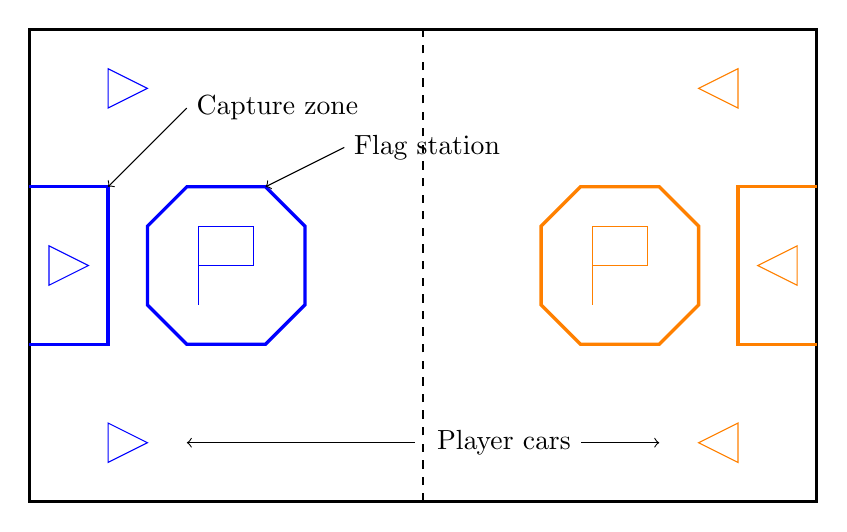
\begin{tikzpicture}

\draw[black, very thick] (-5, -3) rectangle (5, 3);
\draw[black, dashed] (0, -3) -- (0, 3);

% draw the blue base
\draw[blue, very thick] (-5, -1) -- (-4, -1) -- (-4, 1) -- (-5, 1);
\draw[blue, very thick] (-3.5, -0.5) -- (-3, -1) -- (-2, -1) -- (-1.5, -0.5) --
                        (-1.5, 0.5) -- (-2, 1) -- (-3, 1) -- (-3.5, 0.5) --
                        cycle;
\draw[blue] (-2.85, -0.5) -- (-2.85, 0.5) -- (-2.15, 0.5) -- (-2.15, 0) --
            (-2.85, 0);

% draw the blue cars
\draw[blue] (-4, 2.5) -- (-3.5, 2.25) -- (-4, 2) -- cycle;
\draw[blue] (-4.75, 0.25) -- (-4.25, 0) -- (-4.75, -0.25) -- cycle;
\draw[blue] (-4, -2.5) -- (-3.5, -2.25) -- (-4, -2) -- cycle;


% draw the orange base
\draw[orange, very thick] (5, -1) -- (4, -1) -- (4, 1) -- (5, 1);
\draw[orange, very thick] (3.5, -0.5) -- (3, -1) -- (2, -1) -- (1.5, -0.5) --
                          (1.5, 0.5) -- (2, 1) -- (3, 1) -- (3.5, 0.5) --
                          cycle;
\draw[orange] (2.15, -0.5) -- (2.15, 0.5) -- (2.85, 0.5) -- (2.85, 0) --
              (2.15, 0);

% draw the orange cars
\draw[orange] (4, 2.5) -- (3.5, 2.25) -- (4, 2) -- cycle;
\draw[orange] (4.75, 0.25) -- (4.25, 0) -- (4.75, -0.25) -- cycle;
\draw[orange] (4, -2.5) -- (3.5, -2.25) -- (4, -2) -- cycle;

% draw some labels
\draw[<-] (-4, 1) -- (-3, 2) node[anchor=west]{Capture zone};
\draw[<-] (-2, 1) -- (-1, 1.5) node[anchor=west]{Flag station};
\draw[<-] (3, -2.25) -- (2, -2.25) node[anchor=east]{Player cars};
\draw[<-] (-3, -2.25) -- (-0.1, -2.25);

\end{tikzpicture}

\caption{Diagram of the play field before release (not to scale). Obstacles will
be placed in the mid-field area to cause futher mayhem and shenanigans.}
\label{fig:play-field}
\end{figure}

\end{figure}


The capture zones and the flag stations are raised platforms
that the Wacky Racers will drive onto as shown in
Figure~\ref{fig:station-pictures}. They are
fitted with RFID readers, LEDs, and a WiFi connection back to the game
server.

\begin{figure}[H]
    \centering

    \begin{subfigure}{.45\textwidth}
        \centering
        \includegraphics[width=.9\linewidth]{capture_zone.jpg}
        \caption{Capture zone}
        \label{fig:capture-zone}
    \end{subfigure} \qquad %
    \begin{subfigure}{.45\textwidth}
        \centering
        \includegraphics[width=.9\linewidth]{flag_station.jpg}
        \caption{Flag station}
        \label{fig:flag-station}
    \end{subfigure}

    \caption{Capture zone and Flag station from Wacky Racers 2018.}
    \label{fig:station-pictures}

\end{figure}


\section{Technical stuff}

Read this section carefully.  There are clues as to how we mark your
PCBs at the end of the assignment.


\subsection{Version control}

Use version control for everything, or else!  Learning git is a skill
you will not regret.

Your group leader should create a forked copy of the wacky-racers-2019
git project and then add the other group members to the project.  This
can be done by:

\begin{enumerate}
\item Go to \url{https://eng-git.canterbury.ac.nz/wacky-racers/wacky-racers-2019}

\item Click `Fork' button.  This will create a copy of the main repository for the project.

\item Click on the `Settings' menu then click the `Expand' button for
`Sharing and permissions'.  Change `Project Visibility' to `Private'.

\item Click on the `Members' menu and add group members as Developers.

\item Using a bash terminal (or other useful shell), enter the command:

\begin{lstlisting}[breaklines]
  $ git clone --recursive https://eng-git.canterbury.ac.nz/your-userid/wacky-racers-2019.git  
\end{lstlisting}

If you do not want to have to enter your password for every git
push/pull operation, you should set up ssh-keys and use:

\begin{lstlisting}[breaklines]
  $ git clone --recursive git@eng-git.canterbury.ac.nz:your-userid/wacky-racers-2019.git
\end{lstlisting}

\item Add a remote URL for the main repository.
%
\begin{lstlisting}[breaklines]
  $ cd wacky-racers 
  $ git remote add upstream https://eng-git.canterbury.ac.nz/wacky-racers/wacky-racers-2019.git  
\end{lstlisting}
%
Again if you do not want to manually enter your password, you can use:
%
\begin{lstlisting}[breaklines]
  $ cd wacky-racers 
  $ git remote add upstream git@eng-git.canterbury.ac.nz:wacky-racers/wacky-racers-2019.git    
\end{lstlisting}
%
If we add more demo code or tweak the instructions in the main
repository, you can get the updated stuff using:
%
\begin{lstlisting}[breaklines]
  $ git pull upstream master
\end{lstlisting}
\end{enumerate}

\subsection{Components}

\begin{enumerate}
\item We recommend that you use components in the ECE Altium library.  These
are stocked in the SMT lab.  For any other components you may require,
see Scott Lloyd in the SMT lab.

\item The Wacky Racer batteries are Radient Superpax 3000 mA-hr 7.2\,V
  NiMH with male Tamiya power connector.  To preserve the battery life
  it is imperative to not draw current when the battery voltage is
  below 6\,V.
\end{enumerate}


\subsection{Schematics}

\begin{enumerate}
\item Have a look at the
  \href{http://ecewiki.elec.canterbury.ac.nz/mediawiki/index.php/ENCE461_Altium_tutorial}{Altium
    tutorial on ecewiki}.

\item Have a read of the
  \href{http://ecewiki.elec.canterbury.ac.nz/mediawiki/index.php/Schematic_guidelines}{schematic
    guidelines on ecewiki}.

\item Add you and your partner's name to the title block on your
  schematic.

\item Save PDF files of your schematics in your source repository.
  \textbf{Note, when debugging your PCBs, we will not help you until you show us your
    schematic}.

\item We bet that you will not have enough test points to clip an
  oscilloscope probe to.  Do not think you can hold the probe tip
  against an MCU pin.  Ensure you give a meaningful name to the test
  point.  A ground test point is essential for an oscilloscope earth
  clip. Keep this clear of other test points since the clip may short
  against them.  You will probably require at least two ground points.
  
\item Checking the schematic is the most crucial part of the
  assignment.  If the schematic is wrong then your PCB will be wrong.
  So, schematics must be thoroughly checked by another person.

\item Consider fall-back options if you have a problem with your PCB.

  The IMU for the Wacky Hat is tiny and we \textbf{strongly recommend} that you
  provide an alternative connector for connecting the following IMU module:
  \href{https://www.aliexpress.com/item/SPI-IIC-MPU9250-MPU-9250-MPU-9250-9-Axis-Attitude-Gyro-Accelerator-Magnetometer-Sensor-Module-MPU9250/32216818498.html?spm=a2g0s.9042311.0.0.WKvtEm}{MPU-9250 on AliExpress}

  Similarly for the Wacky Hat, in case the H-bridge fails, provide two
  three-pin servo connectors so that external Electronic Speed
  Controllers (ESC) can be used to drive the motors.

\item It would be useful to have a jumper or two connected to a PIO
  pin so that you can configure your board.  For example, if a jumper
  is in, use the joystick, otherwise use the IMU.
  
\end{enumerate}


\subsection{PCBs}

\begin{enumerate}
\item Your four-layer PCBs are going to be manufactured by
\href{http://ecewiki.elec.canterbury.ac.nz/mediawiki/index.php/PCB_Zone}{PCB
  Zone} in Auckland.  They produce a PCB solder mask and plated
through holes.  We will be putting several groups's boards onto a
panel to reduce costs.

\item It is important that you check footprints for parts thay you
  create.  We will impose a 10\% penalty for each rerun of a PCB, say
  due to a footprint mistake.  Get your partner to check.
  
\item PCB layouts must be thoroughly checked by another person.
  
\item A PCB track can blow faster than a fuse. So keep high current
  tracks fat and short.

\item Clearly mark the positive and negative battery connections on
  the silk screen.

\item Some of the chips can get hot so thermal considerations are
  required.  Follow the manufacturers' guidelines in the datasheets.

\item The switching regulators can interfere with the radios.
  
\item Use a design rule check to see if any of the following
  constraints are violated:
%
\begin{itemize}
\item Minimum trace width (0.15\,mm)
\item Minimum trace clearance (0.15\,mm)
\item Minimum via size (0.3\,mm hole, 0.6\,mm outer diameter)
\item Minimum hole size (0.3\,mm)
\item Minimum annular ring (0.1\,mm)
\end{itemize}
%
For every violation of one these rules, we will deduct 1\% from your
final mark.

\item Check the
  \href{http://ecewiki.elec.canterbury.ac.nz/mediawiki/index.php/PCB_checklist}{PCB
    checklist on ecewiki} before submission.
\end{enumerate}


\subsection{Assembly}

\begin{enumerate}
\item Finding shorts is extremely frustrating so maximise clearances
  and test for shorts before populating components.

\item Components can be put through the oven on the reverse side
  although heavy components may need to be glued.
  
\item Never assume where pin 1 is on an IC; check the datasheet.  
  
\end{enumerate}


\subsection{Software}

\begin{enumerate}
\item We highly recommend using a personal laptop with Linux installed if
possible. A virtual machine running on Windows is acceptable for this. You will
need to check instructions on ecewiki for how to install the required toolchain.

\item We do not support embedded systems development on Windows, but is is
possible.

\item If you are not using version control for this you are foolish.

\item Inspect MPH's sample code.

\end{enumerate}


\subsection{Programming}

\begin{enumerate}
\item If you are trying to program the SAM4S for the first time and
  are feeling tired or impatient, then do something else.

\item For the first program, do not use batteries or a USB connection.
  The ST-Link adapter will provide 3.3\,V to the MCU.
 
\item Detailed instructions can be found at
  \url{http://ecewiki.elec.canterbury.ac.nz/mediawiki/index.php/Wacky_racers_software}.
\end{enumerate}


\subsection{Debugging}

\begin{enumerate}
\item Start running small programs (such as the provided demo
  programs) to test each feature separately.
  
\item An oscilloscope is your friend.

\item It is possible to use the GDB debugger but you need to know what
  you are doing, especially with optimised code.

\item Drawing a diagram of what you think is happening is highly recommended. A
simple circuit diagram or timing diagram will often help you realise what you
have missed and let you fix it without asking for help.
  
\end{enumerate}


\subsection{Possibly asked questions with answers}

\begin{itemize}
\item \emph{Why use the SAM4s MCU?}  For this application most MCUs
  would suffice, even an 8-bit AVR microcontroller.  To level the
  playing field, I have chosen a MCU most students would not have used
  before.  This is an ARM based MCU made by Atmel I have used this in
  a number of projects.  Indeed we used to teach in in ENCE361.  There
  are many other similar MCUs made by different manufacturers such as
  the STM32 that would just as suitable.

\item \emph{Why use a four layer PCB?}  Come to lectures to find out!

\item \emph{How was the PCB size chosen?}  This was so twenty boards
  would fit on an A3 panel to reduce manufacturing costs.

\item \emph{Why use 7.2\,V NiMH batteries for the Wacky Racers?}
  These were a legacy of previous Wacky Racers.  They are also safer
  than lithium batteries.

\item \emph{Why can't I program my device using Windows?} Due to various aspects
of the Windows ecosystem, setting up a fully functional build environment is
more complicated, will often vary from machine to machine, will often break
filepaths, and will often cause bizarre compilation errors. Use at your own
risk, we will not assist in debugging issues related to Windows.

\item \emph{Can you please fix my problem for me?} Due to limited TA time
available, we will only provide debugging assistance to students who have a
printed A3 schematic sheet in front of them and have already tried looking up
the problem on the ecewiki.

\end{itemize}

\section{Changelog}

\begin{itemize}
  \item Version 2: removed battery monitoring from the functional assessment
  list. Calrified low battery voltage requirement.

  \item Version 3: loosened the assignment schedule to make term 2 less
  stressful.
  
  \end{itemize}

\end{document}

